\chapter{A Simulation Study of Hardware Parameters for Future GPU-based HPC Platforms}

 In this work, I delve into the issue of optimizing hardware parameters for next-generation GPU-based High Performance Computing (HPC) platforms, specifically addressing the challenges and opportunities presented by integrating multiple GPUs within compute nodes. This is motivated by the evolving landscape of HPC platforms, where there is a marked shift toward increasing computational capacity per node while concurrently reducing the overall number of nodes or endpoints in the system.
Prior studies, such as those by Jain et al. [3], have laid the groundwork by evaluating the performance impact of various fat-tree configurations, offering valuable insights into network architecture's role in HPC systems. Similarly, research on topology and routing methods for Dragonfly networks by Rahman et al. [27] and on Jellyfish topologies by Zaid et al. [28] has advanced my understanding of network performance under different configurations. These studies, while foundational, primarily focus on network topologies and configurations rather than the integrated approach of combining only hardware parameters.
To provide context for this investigation, the increasing significance of compute acceleration devices, such as GPUs, which have drastically altered the computational landscape of HPC platforms. These devices have enabled a substantial increase in the computational capabilities of individual nodes, which is observed in the comparison between Sequoia at LLNL and Summit at ORNL. This transformation warrants a reconsideration of hardware architectural parameters to ensure that future HPC platforms can achieve optimal performance levels.
This study aims to address the imbalance between computation and communication capacities that arises as there is an ongoing transition to HPC systems with fewer, more powerful nodes. The integration of multiple GPUs per node introduces new complexities in maintaining an efficient computation-to-communication ratio, making it imperative to explore hardware configurations that can mitigate these challenges.
To tackle these issues, this study utilizes the TraceR-CODES simulation tool to analyze the impact of various hardware design parameters on the performance of realistic HPC workloads. This investigation centers on three critical hardware parameters: the number of GPUs per node, network link bandwidth, and network interface controller (NIC) scheduling policies. These parameters are evaluated within the context of two widely-used network topologies: fat-tree and dragonfly.
The main conclusions of this study underscore the nuanced relationship between hardware parameters and system performance. The results show that the optimal configuration of GPUs per node, network bandwidth, and message scheduling strategies significantly depends on the specific demands of the applications running on the HPC platform. For instance, communication-intensive applications may require higher network bandwidth to maintain performance levels as the number of GPUs per node increases. Conversely, computation-heavy applications may see minimal impact from changes in network bandwidth but could be affected by NIC scheduling strategies. 


In summary, this work contributes to the ongoing process of optimizing HPC platforms for the era of GPU acceleration, offering insights that can inform both the design and implementation of future systems. By bridging the gap between computational capacity and communication efficiency, this research aims to pave the way for more powerful, efficient, and capable HPC platforms.

\section{Validation of Tracer-CODES}

TraceR-CODES has been previously validated with micro-benchmarks and stand alone
applications including pF3D, 3D Stencil, ping-pong, all-to-all,
etc~\cite{Jain:sc2017}. These validation studies were done for fat-tree networks
and it was found that TraceR-CODES predicts the absolute value as well as the
trends in the execution time with less than 15\%
error~\cite{Jain:sc2017,acun:padabs2015}.  However, these validation studies 
have been done with single job simulations. Further, these studies did not
validate cross-platform and cross-network projections, i.e. traces were
collected and projections were done for the same system.

To gain confidence in TraceR-CODES' prediction for cross-platform and
cross-network multi-job workloads as well
as in the new additions to TraceR-CODES, this work validates TraceR-CODES with three random
multi-job workloads.
The validation is done by 1)~randomly creating three workloads that consist of 
representative HPC benchmarks with different communication and computation
characteristics, 2)~running the workloads on the Quartz supercomputer~\cite{quartz} at LLNL,
3)~simulating the workloads using TraceR-CODES with the system parameters
set to the values for Quartz, and 4)~comparing the predicted job execution
times from the simulations with the measured times on Quartz. 

The three workloads are formed by selecting jobs from two communication intensive
benchmarks (Stencil4d and Subcomm3d) and two computation intensive applications
(Kripke and Laghos). More information about the applications is given in
section ~\ref{applicationworkload} 

In this study, three workloads were run in a dedicated access time (DAT) on Quartz at LLNL, during this period
no other jobs ran on the machine. It used linear mapping of job
ranks to nodes and measured the execution time of each job in the workloads.
For simulation with the TraceR-CODES framework, it used the
exact system settings as Quartz: (1)  create
the exact fat-tree topology as Quartz using the arbitrary graph model; (2)
 set the values of the network parameters to the corresponding values on Quartz:
11.9 GB/s peak link bandwidth, 8 packets buffer size, 4096 bytes packet size,
and so on; and (3) the jobs and processes in each workload
are mapped to compute nodes exactly in the same
way as they ran on Quartz. 

The traces for driving the simulation were collected on
Vulcan~\cite{vulcan}, a 5D-torus based Blue Gene/Q
system.  Since the computational capabilities of Vulcan are different from
Quartz, the relative compute scaling factor between Vulcan and
Quartz is calculated, and the computation regions of simulations were scaled accordingly. This
setup helps to evaluate the projections when the network (5D-torus vs fat-tree)
as well as computational capability (IBM PowerPC vs Intel Xeon) of the traced
system are different from the target system.
%Finally, I use the exact job and node mapping in the simulation as the real
%job when run on Quartz. 

\begin{figure}[h]
  \centering
  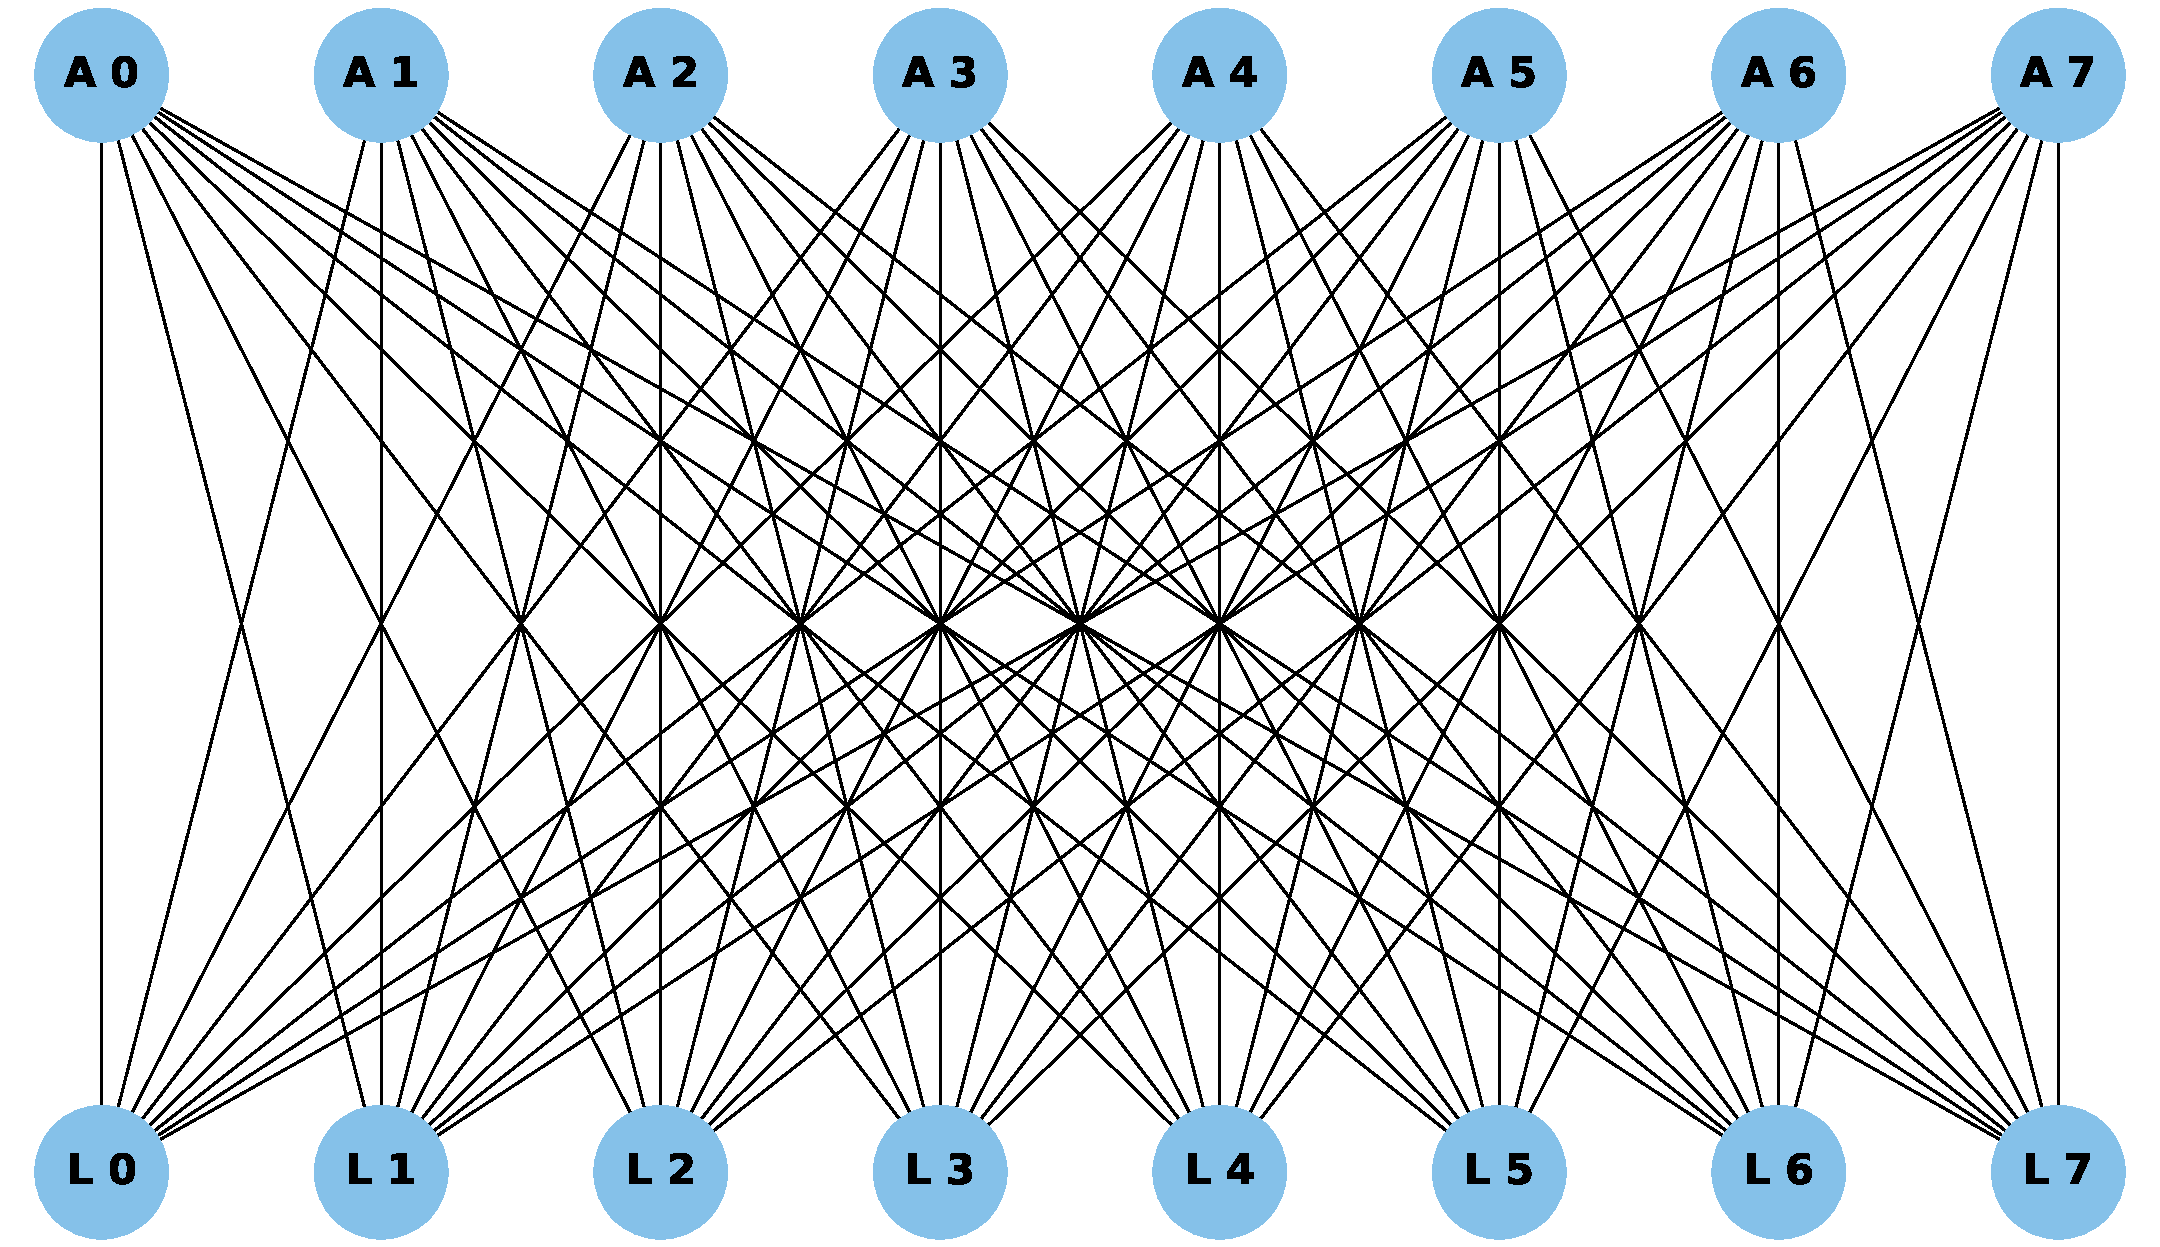
\includegraphics[width=0.8\columnwidth]{figure/val/quartztopo.pdf}
  \caption{A Quartz pod with eight aggregate and eight leaf switches, and all links.}
  \label{fig:quartz_pod}
%\end{multicols}
\end{figure}

\vspace{0.08in}
\noindent{\bf Quartz Topology:} The Quartz system deploys a 3-level fat-tree, with a 2:1
tapering at each of its 84 leaf switches. There are 84 aggregate switches and 32
core switches. Each switch has a radix of 48 and each leaf level switch is
connected to 32 compute nodes.  Note that some ports in the aggregate switches
and core switches are left unused.  The 84 leaf level switches are divided among 
11 pods. Figure~\ref{fig:quartz_pod} shows a Quartz supercomputer pod.  Each pod consists 
of 8 leaf switches and 8 aggregate switches, which are connected in an
all-to-all bipartite graph. Each arc drawn here represents two physical links. 
In contrast, a standard 2:1 tapered fat-tree would have 16 leaf switches in 
each pod, which are connected to 16 aggregate switches using one physical link
each. We give these details of the Quartz topology to highlight that
Quartz' fat-tree is different from the standard, symmetric fat-tree topology,
as are the networks in most production systems. These differences are the main driver
for the development of the {\em arbitrary graph model}. 

Figure~\ref{fig:validation} shows the results of the validation. The
horizontal axis, have each application and their corresponding job size used
in various workloads. Each blue dot represents the average 
of the error percentage between the predicted runtime and the measured runtime
for various
instances of the given application-job size pair that appear across the three workloads. For
example, since Subcomm3d jobs with a process count of 128 appears two times
across the three workloads, their average error percentage is computed to be
-7.88\%. It can be observed, that for all cases except 32-ranks
Stencil4d, the prediction error is within 20\%; and for all except 3 cases
(32-rank Stencil4d, 32-ranks Kripke, and 64-ranks Kripke), the error is within 15\%.
These results suggest that TraceR-CODES predictions reasonably approximate 
the actual runtime on real systems for multi-job workloads even when the
computational capability and underlying network are different.

\begin{figure}[h]
\centering
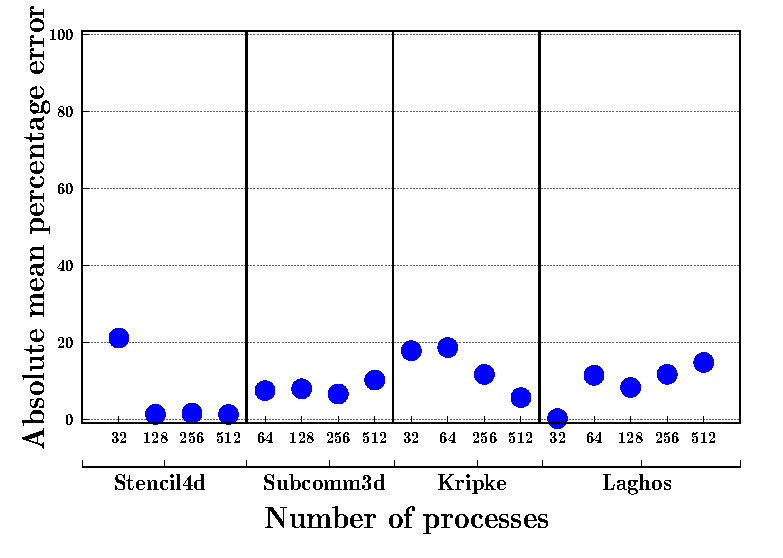
\includegraphics[width=\columnwidth]{figure/val/quartz.eps}
\caption{Validation of TraceR-CODES (mean percentage error in predicted runtime compared to the actual runtime).}
\label{fig:validation}
\end{figure}



\section{Simulating Message Scheduling in the NIC}

The network interface controller (NIC) in contemporary HPC systems is
responsible for scheduling and packetizing messages.

\vspace{0.08in}
\noindent{\bf FCFS scheduling:} 
Messages are inserted
at the back of the scheduling queue, as and when they arrive.
During the packetization process, %the scheduler pops the elements from the head of
%the scheduling queue, creates the packet from that message, and pushes it back
%to the top.
the scheduler keeps creating packets from the top of the queue until
the entire message is packetized before it packetizes the next message in the queue. 
%This is what typically happens when there is
%only one virtual channel in a NIC/network.

\vspace{0.08in}
\noindent{\bf RR scheduling:} Messages are inserted into the scheduling queue of
the network interface, as and when they arrive. During the packetization process,
the scheduler creates one packet for a message and then moves to the next message:
all messages are considered in a round-robin manner. 
%However during the packetization process, the scheduler pops the top message from
%scheduling queue, creates a packet from it and then inserts to the tail. The scheduler
%then moves to the next message in the queue, which is currently at the top of the
%scheduling queue. The scheduler repeats the process until all the messages in the
%scheduling queue are packetized before it again creates a packet from the first message
%which entered the queue initially.
RR not only allows concurrent communication
progress for several communicating-pairs, but may also help the network in
better utilizing multiple communication paths. While desirable, such a scheme is
difficult to implement in the hardware as the number of concurrent messages can
be very large.

%default first come first serve (FCFS) message
%scheduling. 
\vspace{0.08in}
%In RR-N, the messages are entering the scheduling queue in the network interface
%in a first come first serve manner with the first N message in the queue, waiting
%for their turn of packetization. Each of those N messages is first packetized one
%after the other. When one of the N messages is completely packetized, the immediate
%next message in the queue takes its place. 

\vspace{0.08in}
\noindent{\bf RR-N scheduling:} In this scheme, $N$ is a parameter. RR-N is similar to RR,
except that instead of packetizing every message in the scheduling queue in
a round-robin manner,
the scheduler packetizes the top $N$ messages in the scheduling queue. For example,
in RR-2, the scheduler only packetizes the first 2 messages for communication.
This newly added scheme simulates the real world scenario where a limited
number of hardware queues are available at a NIC, which are used to keep
multiple message in-flight concurrently.
%and thus
%packetization of only these many messages can happen concurrently.  



\section{Hardware Design Parameters}
\label{sec:hardwareparameters}
\vspace{0.08in}
\noindent{\bf Network topology:}
In this study's experiments, the impact of the hardware design parameters are studied in the context of two 
widely used interconnect topologies: fat-tree and 1D dragonfly.
%Both topologies are used in the current and future HPC systems. 

{\em (1)~1D Dragonfly} -- 1D Dragonfly \cite{Kim2008ISCA}
is a two-level direct network topology: switches form groups with a fully connected
intra-group topology and groups are connected with an inter-group topology.
The topology has three important parameters \cite{Kim2008ISCA}:
the number of compute nodes in each switch ($p$),
the number of links in each switch that connect to other switches in the same group
($a$), the number of links in each switch that connect to other groups ($h$). A balanced dragonfly
in general requires $a = 2p = 2h$. In this study the parameters are set to $p = h = 8$ and $a = 16$.
Each group has 16 switches and 128 compute nodes. 
The global link connectivity between groups follows the per-router arrangement
%with parameters
%(8,1,1) as specified in
\cite{Alzaid2020ICS}.
%For one GPU per node system, the network has
%16 groups and 2048 compute nodes. The number of groups is reduced as more GPUs are
%equipped on each compute node: there are 8 groups
%for 2 GPUs per node case, 4 groups for 4 GPU per node case, and so on. 
The routing algorithm used is the progressive adaptive routing (PAR) \cite{Kim2008ISCA,Alzaid2020ICS}.
% Figure~\ref{fig:dfly_group} show the link connectivity from router R0 in our 1D Dragonfly topology.

{\em (2)~Fat-tree} -- The other topology is a 3-level full bisection bandwidth
fat-tree.  In a 3-level full bisection bandwidth fat-tree, there are three types
of switches: 1)~core switches which are at the top layer to connect pods,
2)~aggregate switches, which connect the leaf switches and form a pod, and
3)~the leaf switches, which are connected to the compute nodes. In a 3-level
full bisection bandwidth fat-tree, the number of uplinks in the aggregate and
leaf switches is the same as the number of downlinks. For our study, the 3-level
fat-tree is built using 32 radix switches. Each leaf switch connects to 16
compute nodes and 16 aggregate switches. Each pod has 16 aggregate switches, 16
edge switches, and 256 compute nodes.
%There are 8 pods in the topology to
%support 2048 compute nodes for 1 GPU per node case, 4 pods for 2 GPU per node
%case, and so on.  We assume adaptive routing for routing of the packets. 

%Figure~\ref{fig:ftree_pod} shows  a fat-tree pod I are use in our
%experiments. We shows the links for L0 and L15 (first and the last leaf
%switch in the pod) and A0 and A15 (first and the last aggregate switch in the
%  pod) to avoid visual clutter. 

\vspace{0.08in}
\noindent{\bf Number of GPUs per node:}
In this study, the number of GPUs in each compute node varies from 1 to
8 to analyze the impact of the increased computation density and the reduction
of network endpoints on the system performance. Each GPU is assigned
to one MPI processes; to simulate different number of GPUs
per node, multiple MPI process are assigned to a node.
The GPUs inside a node are connected in an all-to-all connection topology resembling the intra node connectivity of the Sierra system with NVlink.
The bandwidth between GPUs within a node
is set to be twice the network link bandwidth, so that it replicates that of Sierra supercomputer.
The default setting for GPUs per node is 1 GPU per node. This is the default
GPU per node setting whose performance is used to normalize other results. 
%to which I compare other results.

In the experiments, when I increase the number of GPUs per node, I
proportionally reduce the number of network endpoints, i.e. I make sure that
for all network configurations, the total GPU count, as well the total MPI
  processes, is 2048. This is done
  to ensure that I compare systems that are of computationally equal capability
  as is often the case in the real world. Secondly, I make sure that each
  workload covers the entire network and no node is left empty during the
  simulation. 
  %Note that these configurations were not used for validation
  %purpose, since the validation was done using the exact Quartz supercomputer
  %topology.  
  Table~\ref{table:configs} summarizes the network sizes used for each GPU
  per node setting, with the default setting being that of 1 GPU per node.  

\begin{table}[h]
       \centering
\caption{Network sizes for different GPUs per node.}
        \vspace{-1em}
        \begin{tabular}{ccc} \toprule
        \textbf{GPUs per node} & \textbf{1D Dragonfly} & \textbf{Fat-tree}\\ \midrule 
        1 & 16 Groups & 
        8 Pods \\
        
        2 &
        8 Groups & 
        4 Pods \\
        
        4 & 4 Groups & 
        2 Pods \\
        
        8 & 
        2 Groups & 
        1 Pods\\ \bottomrule
        \end{tabular}
\label{table:configs}
\end{table}

\begin{figure*}[t]
\centering
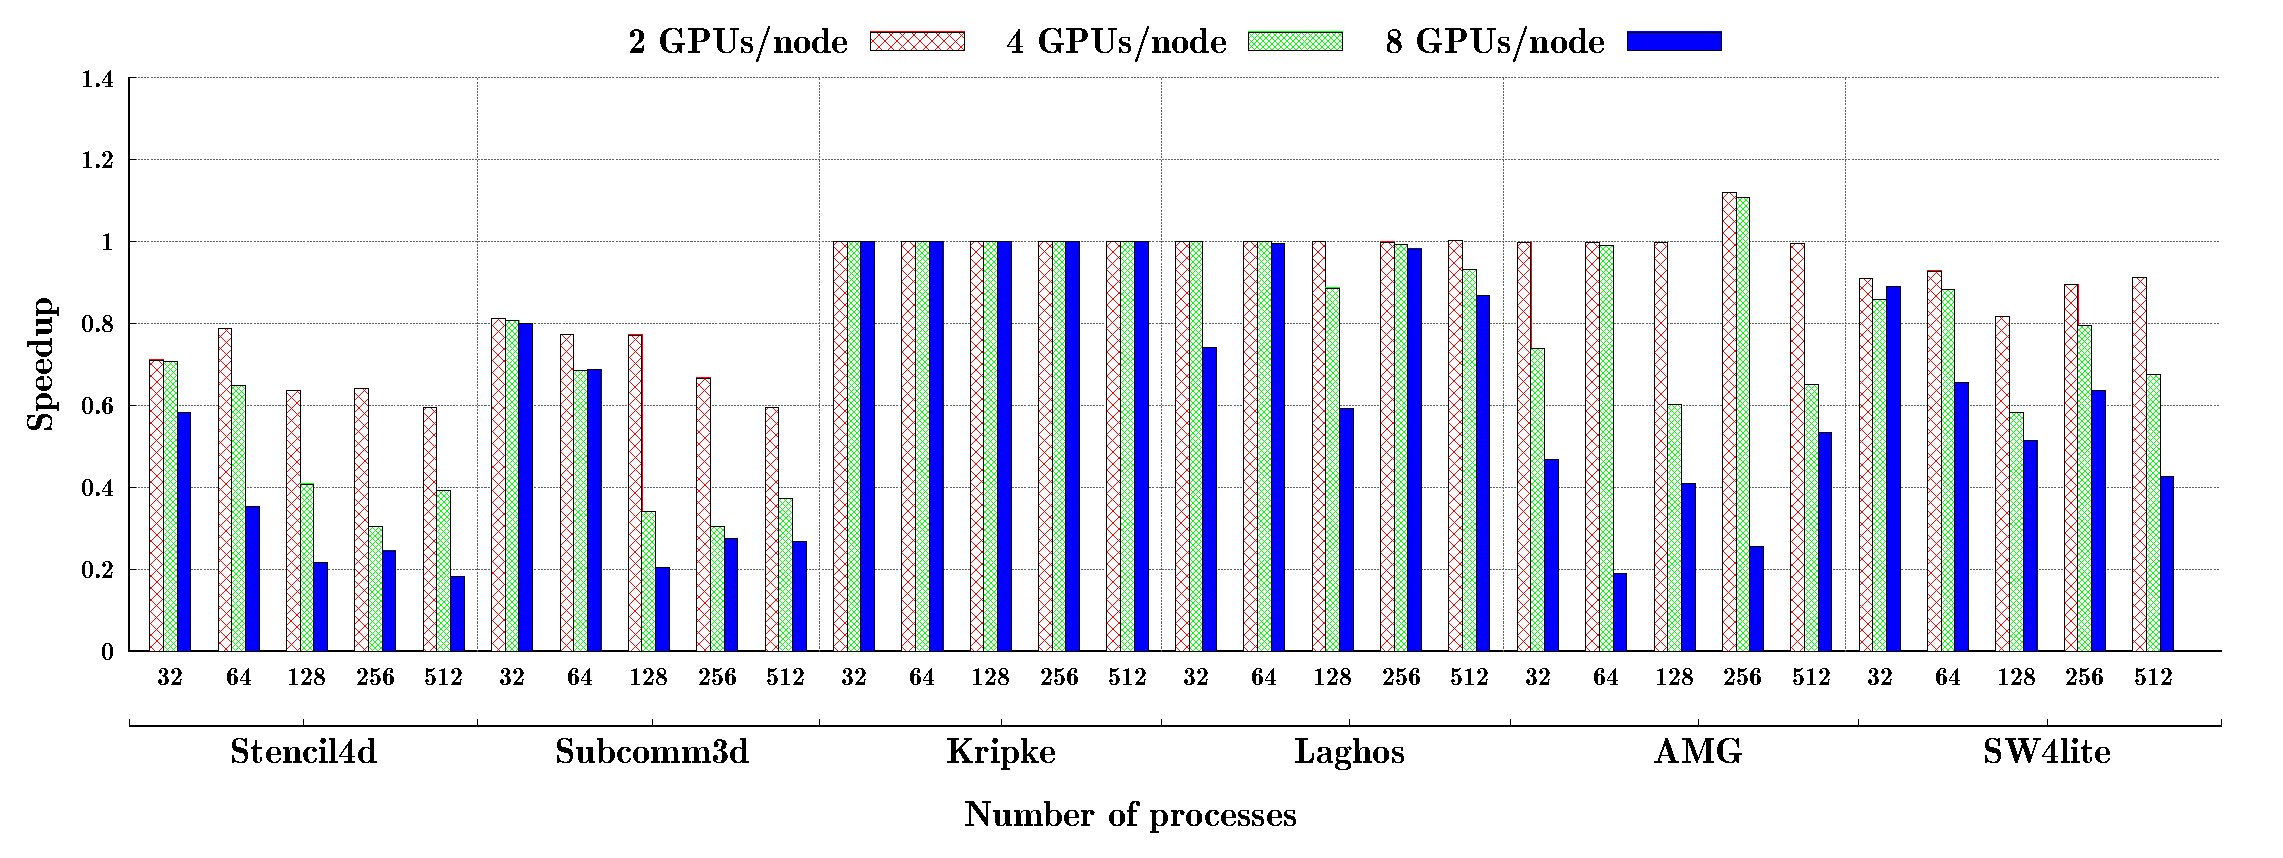
\includegraphics[width=\textwidth]{plots/ftree/map/ftree-mapping-all.eps}
\caption{Speedup on fat-tree for various numbers of GPUs per node settings with
respect to 1 GPU/node configuration.}
\label{fig:ftree_gpu}
\end{figure*}

\vspace{0.08in}
\noindent{\bf Network link bandwidth:}
We set our baseline link bandwidth as x=11.9 GB/s, which is the peak achieved
link bandwidth on Mellanox EDR networks such as
the Quartz supercomputer at LLNL. To analyze the
sensitivity of various compute capability equivalent systems to communication capability, I vary the bandwidth
from x/16 (16 times slow down of the baseline) to 16x (16 times speedup of the
baseline). In the rest of the paper, I will use x to represent the base
bandwidth, and will denote the network speed as x/16, x/8, x/4, x/2, x, 2x, 4x,
8x, and 16x.  
%Varying the network speed allows us to quantify the impact of
%increasing network bandwidth for various compute capability equivalent systems.


\vspace{0.08in}
\noindent{\bf Message scheduling:}
As the computation and communication density
on the compute node increases, message scheduling performed by the
NIC may have an impact on
communication performance. In particular, scheduling schemes that alleviate
head-of-line blocking may have significant benefits, especially when the link
bandwidth is very high. In addition to head-of-line blocking, which is often mitigated
by the use of virtual channels, message scheduling also affects congestion management and network
utilization. Scheduling schemes that expose packets from multiple communicating-pairs
to the network may perform better as it provides the network with the flexibility to
use multiple network paths concurrently. To investigate the effect of message scheduling
on a system with different network and different node compute capability, I compare the performance
of FCFS, RR, and RR-N with different values of $N$ on systems with different configurations. 




\section{Application and Workloads}
\begin{figure*}[t]
  \centering
  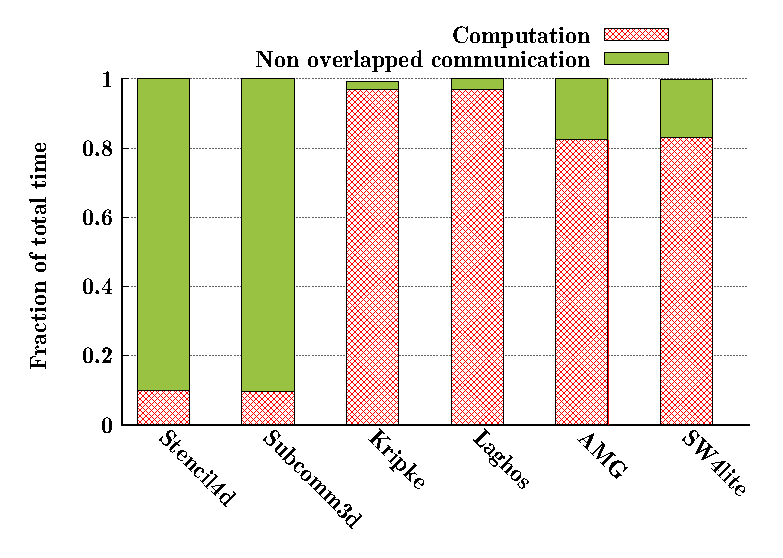
\includegraphics[width=0.8\columnwidth]{figure/val/mpi-scaled.eps}
  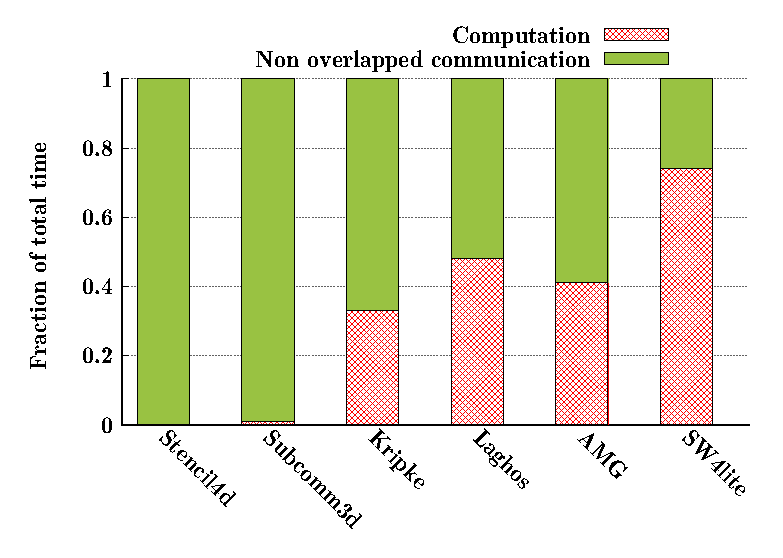
\includegraphics[width=0.8\columnwidth]{figure/val/mpi.eps}
  \caption{Computation and communication characteristics of all applications without scaling (left) and with scaling for GPUs (right)
running on 32 processes.} 
  \label{fig:trace_profile}
\end{figure*}


% The experiment has two components. First, I validate the TraceR-CODES
% framework by comparing simulation results with measurement results on a real
% supercomputer. Second, I study the impact of the hardware parameters on the
% performance. In the following, I will give details about our experiment
% design and configuration.

\label{sec:applicationworkload}

I selected six applications of different computation and communication
characteristics to create realistic HPC workloads. The applications include two
communication-heavy kernels, Stencil4d\cite{bhatele2018evaluating} and Subcomm3d\cite{bhatele2018evaluating}, two compute-intensive
applications, Kripke\cite{kripke} and Laghos\cite{laghos}, and two applications with a balanced
communication-to-computation ratio, AMG\cite{amg} and SW4lite\cite{sjogreen2018sw4} (see
Figure~\ref{fig:trace_profile}).  The traces used in the study were
collected using Score-P \cite{knupfer2012score} on Vulcan, a Blue Gene/Q
installation and Quartz, an Intel Xeon cluster at Lawrence Livermore National
Laboratory (LLNL). The traces contain information about all MPI events executed on each MPI process, along with their
timestamps. In addition, they also record user annotations such as loop
begin and end for the main compute loop. A brief description for the applications in provided in Chapter 2. 


\begin{comment}
Following
is a brief description of the six applications:

\begin{itemize}
\item \textbf{Stencil4d}: MPI benchmark with 8-point near-neighbor communication in a 4D virtual process grid.
\item \textbf{Subcomm3d}: MPI benchmark with all-to-all communication within subsets of processes in a 3D virtual process grid.
\item \textbf{Kripke}: 3D $S^n$ deterministic particle transport code, which runs an
  MPI-based parallel sweep algorithm.
\item \textbf{Laghos}: Proxy application that solves time-dependent Euler equations with MPI-based
  domain decomposition.
\item \textbf{AMG}:  Parallel algebraic multigrid solver.
\item \textbf{SW4lite}: Proxy application for SW4~\cite{sjogreen2018sw4}, a 3D seismic modeling code.
% The computational domain is discretized on one Cartesian mesh and optionally
% on one curvilinear mesh that follows a simple topography.
\end{itemize}
\end{comment}

Figure~\ref{fig:trace_profile} presents the fraction of total execution
time these applications spend in communication and computation when running
with 32 processes.  Computation is denoted by the red color, and non-overlapped
communication is shown in green. At 32 processes, Stencil4d and Subcomm3d are
dominated by communication. The communication-computation ratios were tuned in
Stencil4d and Subcomm3d such that they replicate the runtime profiles of
representative communication-intensive applications.  Kripke and Laghos are
dominated by computation with both spending more than 95\% of the time in computation.
AMG and SW4lite spend $\sim$80\% of their time in computation and the rest in
communication.  Suitable
computation scaling factors are used to alter the behavior of these traces to
emulate running the computation on GPUs. Figure~\ref{fig:trace_profile} 
shows how the computation-to-communication ratios change as these
scaling factors are applied. Stencil4d and Subcomm3d spend most of their time in
communication after compute scaling and the other applications now spend
between 25-65\% in communication.

The workloads in the study are created using the six HPC applications mentioned
above at different process counts -- 32, 64, 128, 256, and 512.  In this study,
the system supports up to 2048 processes. Thus, the sum of process counts in
each of the workloads is exactly 2048.  Each workload is obtained by
iteratively randomly selecting an application and a job size until the total
workload size has reached 2048.  As a result, each workload has many jobs of
different sizes, resembling the capacity workload of supercomputing
centers~\cite{jain2016evaluating}.  This study's experiments use 20 such random
workloads. To ensure that the reported performance of each job size of each
application is representative, each job size of each application
appears at least four times in the 20 workloads. This warrants that each job
size of each application has been executed under different conditions in the
experiments.
 


\section{Performance Study}
\begin{figure*}[t]
\centering
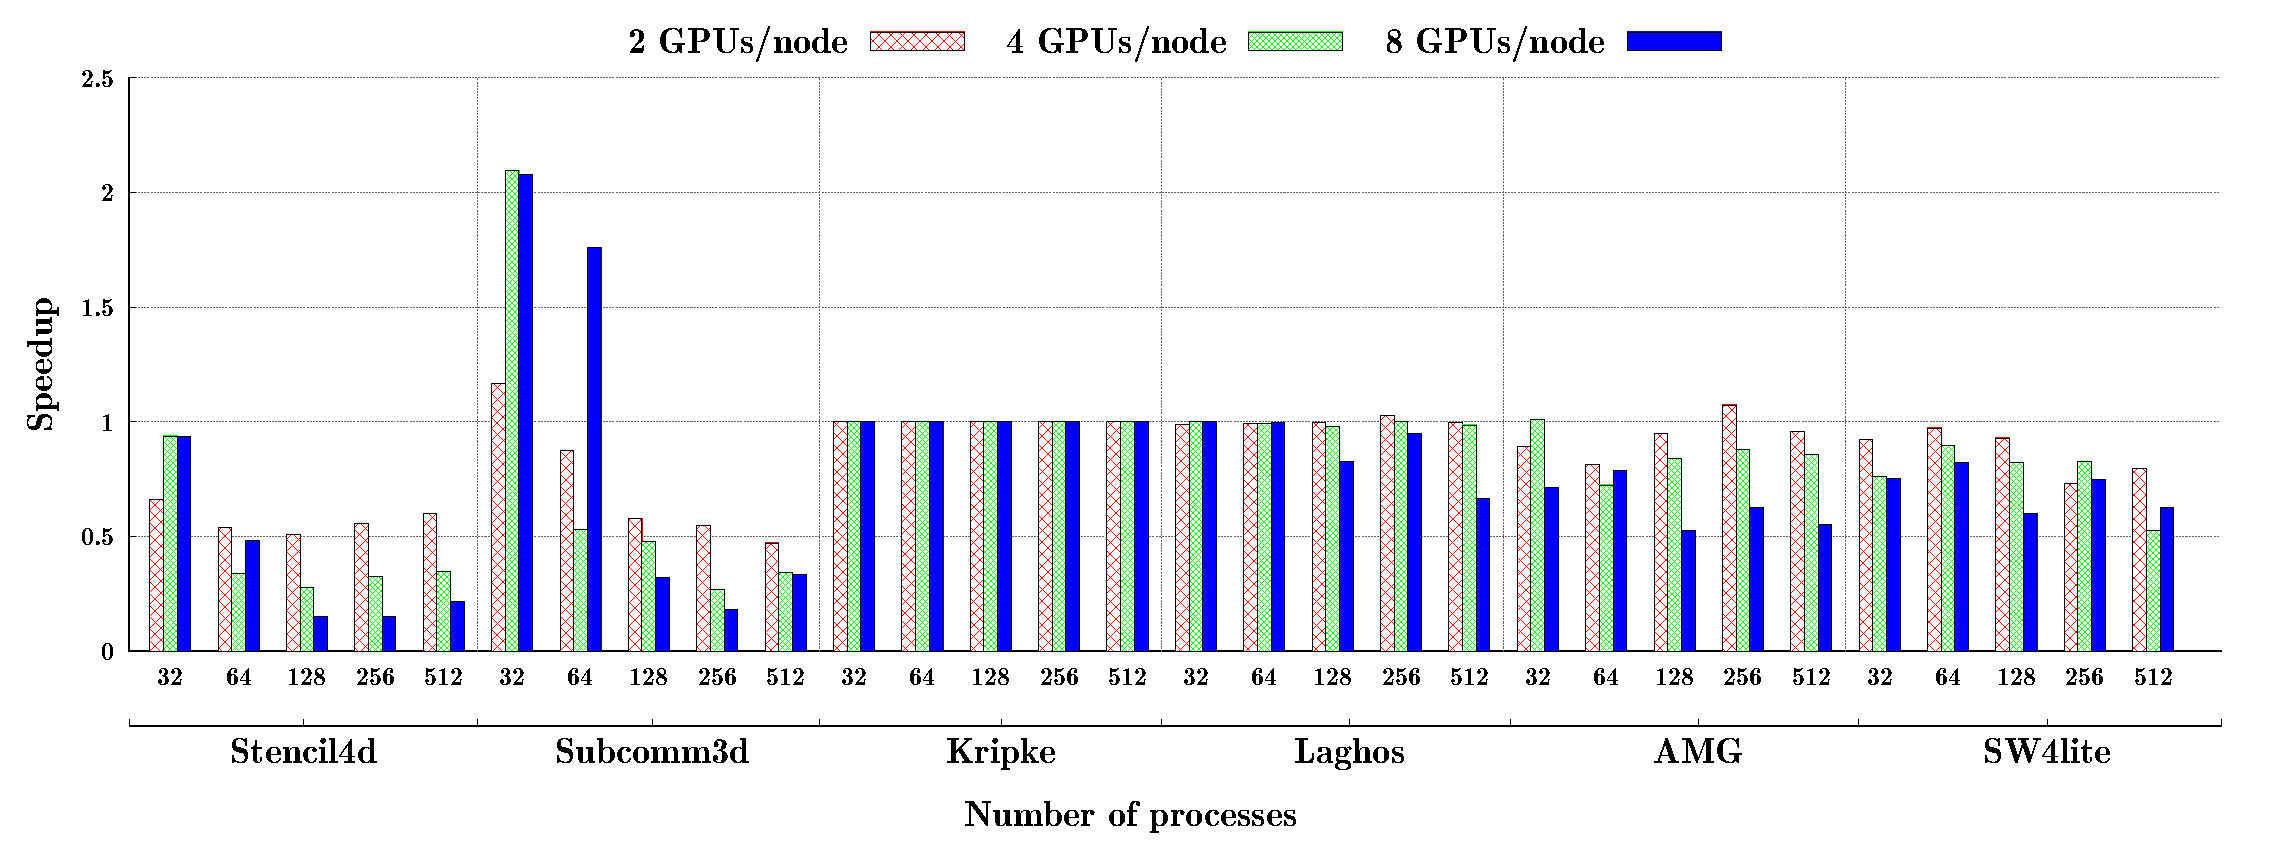
\includegraphics[width=\textwidth]{plots/dfly/map/dfly-mapping-all.eps}
\caption{Speedup on 1D dragonfly for various numbers of GPUs per node settings with
respect to 1 GPU/node configuration.}
\label{fig:dfly_gpu}
\end{figure*}


We now present the results of simulation studies that vary
different architectural parameters presented in
Section~\ref{sec:hardwareparameters}.

\subsection{Impact of the number of GPUs per node}

The number of GPUs per node determines the balance of computation 
to communication capacity of a system and thus is an important configuration
choice in GPU-based HPC clusters. We study
the impact of this parameter on different types of HPC applications.

Figure~\ref{fig:ftree_gpu} presents the relative performance of the applications
running on fat-tree based systems with different number of GPUs per node.  The
speedup in the figure is computed relative to the performance when running with 1 GPU per node.
For example, in Figure~\ref{fig:ftree_gpu}, Stencil4d with 32 processes has a
speedup of 0.71 in the 2 GPUs per node mode. This implies that the performance
of Stencil4d with 2 GPUs per node is 71\% of the Stencil4d performance with 1 GPU
per node.  Other configuration parameters are held constant at their default
values (1x network link bandwidth, FCFS message scheduling, etc.) The
reported performance is the average across all occurrences of an application
and a given job size in the 20 workloads. Note that across the different GPUs per node
configurations, each application and job size combination gets exactly the same computing
resources. More GPUs per node does not imply more computing power for a given
application and job size combination; it simply implies that the computing resources are
available in a more condensed manner on fewer, more powerful nodes.

In Figure~\ref{fig:ftree_gpu}, I see that for communication-heavy
applications (Stencil4d and Subcomm3d), as the number of GPUs per node
increases, application performance drops for most job sizes. This is because
as more GPUs are placed per node, the effective communication resources
available for each GPU reduce. However, the performance drop is not linear
w.r.t.~the effective communication resources because the mapping of multiple
MPI processes to node results in some of the data being communicated within
node. This data can make use of the high-bandwidth intra-node GPU links.

An opposite effect is observed in the simulations of the 1D dragonfly
topology in Figure~\ref{fig:dfly_gpu}. In some cases, such as Subcomm3d on
32 and 64 nodes, a significant amount of traffic is converted to intra-node
when using 8 GPUs/node, which results in performance improvement of the
application.  Another factor that impacts performance is that when all
processes in a job are mapped to a single switch, the job is less
susceptible to inter-job network interference than when the processes in a
job are mapped to multiple switches in the interconnect.  With 4 GPUs per
node, a 32-process job is mapped to 8 nodes and a 64-process job is mapped
to 16 nodes.  With 8 GPUs per node, a 32-process job is mapped to 4 nodes
and a 64-process job is mapped to 8 nodes.  Each switch in the fat-tree
connects to 16 nodes and each switch in 1D dragonfly connects to 8 nodes:
there are chances for the 32-process and 64-process jobs to be mapped
completely within one switch and achieve higher performance.  

For the next two applications (Kripke and Laghos), I observe a noticeably
different impact of changing the balance of communication to computation
capability. In the case of Kripke, more GPUs per node do not impact its performance. This
is because the overall communication volume is low, and GPUs are often waiting
on other GPUs to finish their computation. For Laghos, I observe a
slowdown primarily with 8 GPUs per node. This indicates that having these many
GPUs per node shifts the communication-computation balance and also the performance 
characteristics of the application.

Finally, for the last two applications (AMG and SW4lite), I observe a gradual
slow down when more GPUs are incorporated per node, on both network topologies. While this performance drop
is not as high as the communication-heavy applications, it is noticeable for the 4
and 8 GPUs per node configurations.  We also find that for most
applications that are sensitive to network performance, several factors
including the communication pattern of the application, job mapping, and
inter-job interference impact the execution time. For example, AMG and Laghos,
experience higher slowdown in 8 GPUs per node configuration in workloads in
which they are placed adjacent to communication-heavy applications. 
The typical reason for
this slowdown is that communication-sensitive applications when mapped
adjacent to similar applications contend for network resources, thus impacting
the performance.

%Figure~\ref{fig:dfly_gpu} shows the results of similar experiments performed for
%systems with the 1D dragonfly topology. We find that the trends for the 1D
%dragonfly topology are similar to that of the fat-tree topology.  Our study with
%different applications and different numbers of GPUs per node, however, reveals
%the general trend when more GPUs are equipped in each node. 


\vspace{1em}
\noindent
{\it \textbf{Overall Observation}:
Most applications run slower with four or more GPUs per network endpoint.} 

\noindent In our experiments, all but one application (Kripke, which is not
sensitive to network capabilities) slow down noticeably with four or more GPUs per network
endpoint.
Although part of the communication volume may be restricted to intra-node communication
with more GPUs per node, this benefit is typically overshadowed by performance
loss due to the reduction of the node communication to computation ratio.  
%With
%the higher GPUs per node setting, applications that have significant
%communication, as well as applications that are placed adjacent to communication
%intensive applications in a workload, will suffer performance degradation.  


%\begin{figure}[h] \begin{multicols}{3} \vspace{-0.6in}

%    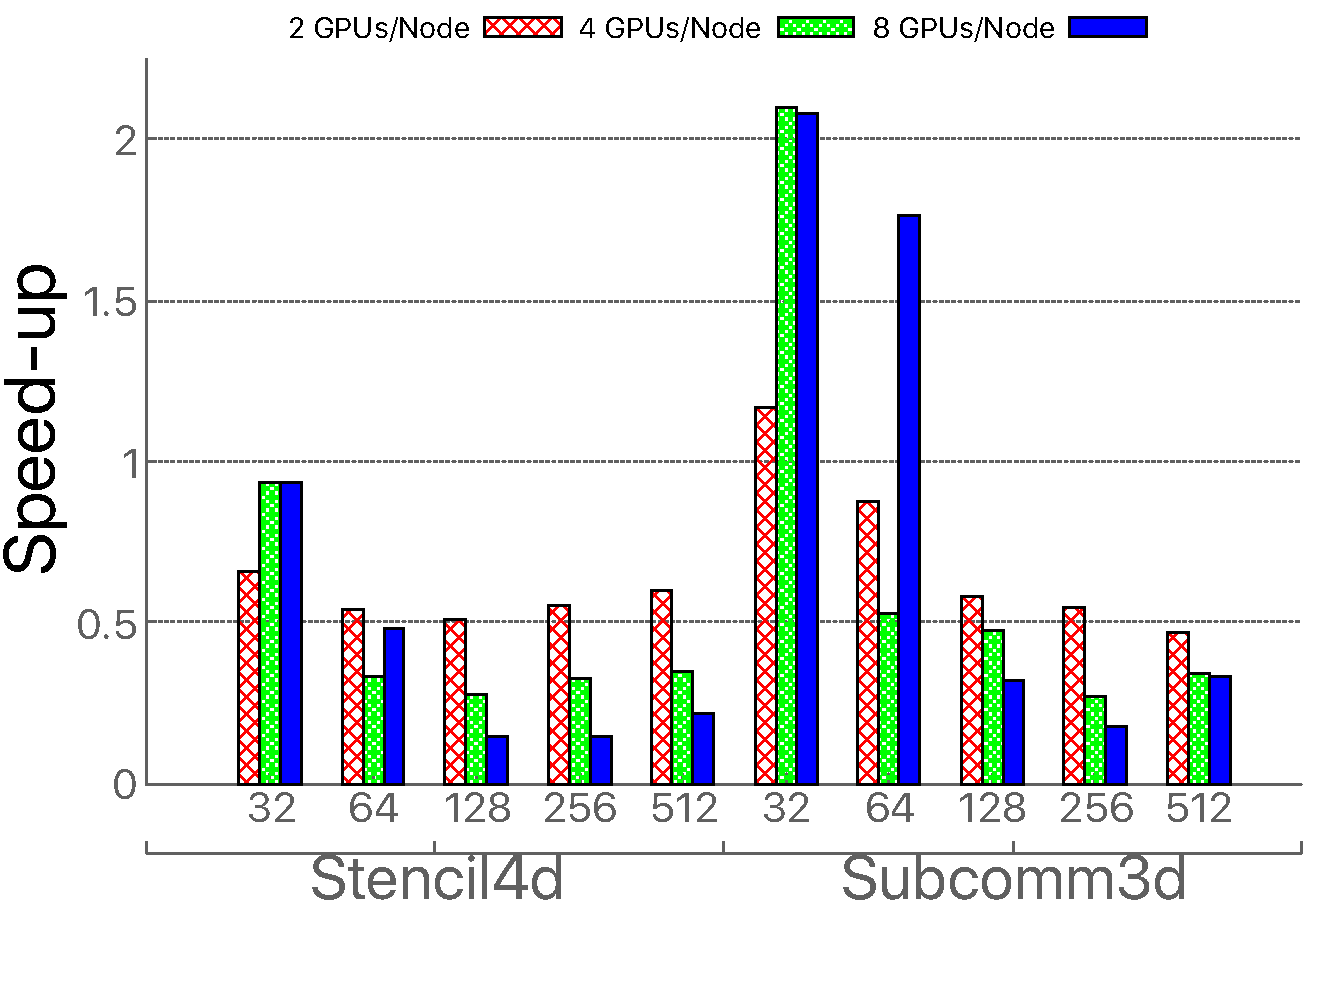
\includegraphics[width=0.8\linewidth]{plots/dfly/map/dfly-x-mapping-comm.pdf}
     % \vspace{-1in}

%  \caption{Performance of communication intensive kernels
%    on 1D dragonfly with default setting and different numbers of
%    GPU's per node}
%  \label{fig:dfly_gpu_comm}
%\end{figure}

%\begin{figure}[h]
    %\vspace{-0.6in}

%    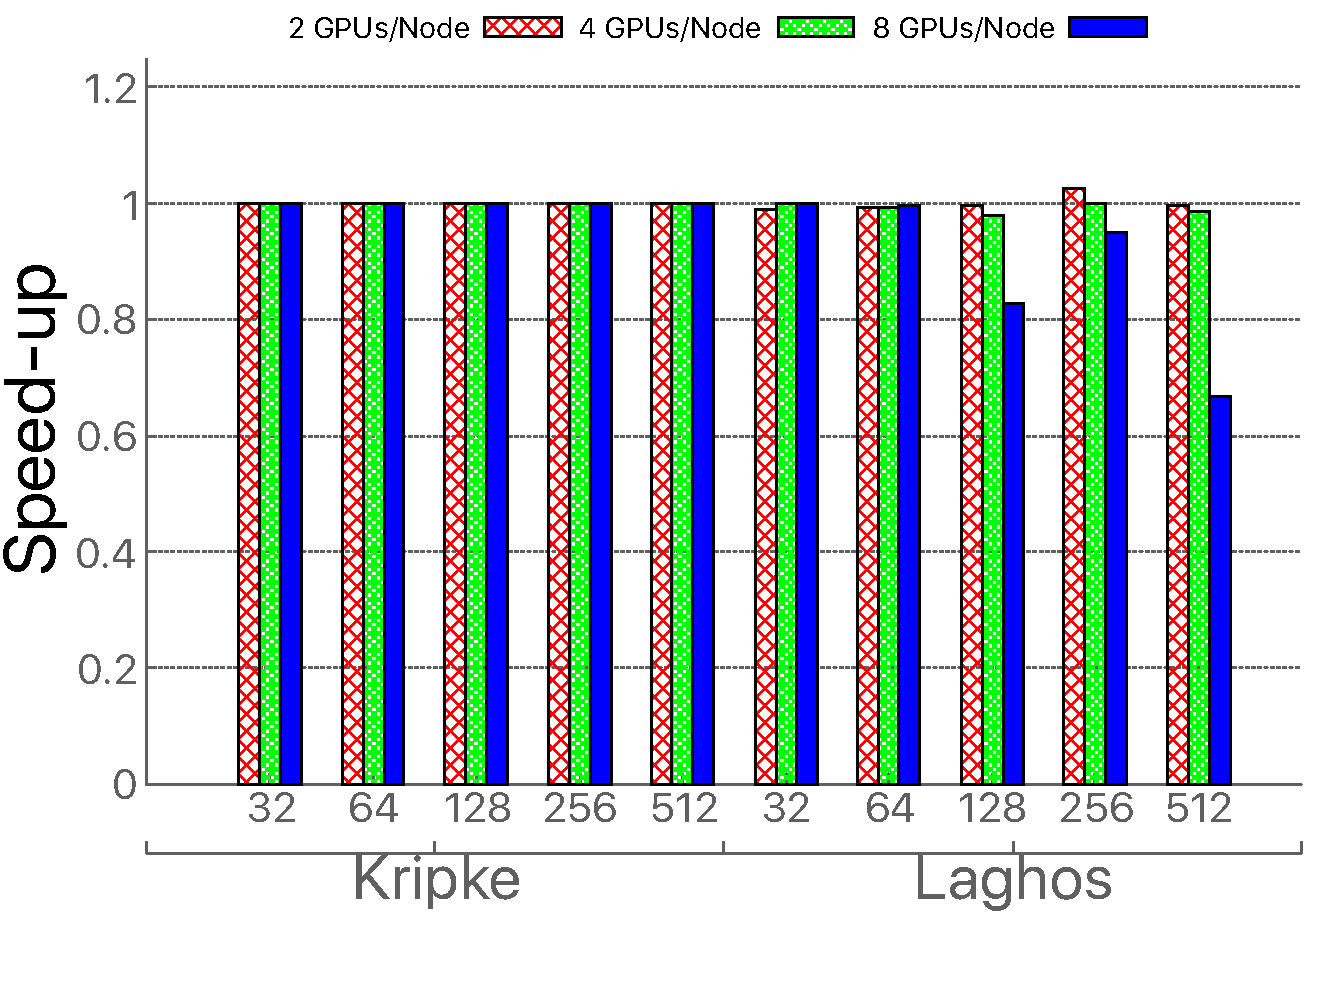
\includegraphics[width=0.8\linewidth]{plots/dfly/map/dfly-x-mapping-comp.pdf}
     % \vspace{-1in}

%  \caption{Performance of computation intensive applications
%    on dragonfly with default setting and different numbers of
%    GPU's per node}
%  \label{fig:dfly_gpu_comp}
%\end{figure}


%For applications where the communication is less intensive, the
%number of GPUs per node affect the applications in different ways
%depending on the intensity of the application. 
%Figure~\ref{fig:mapping_comp_fcfs_ftree} shows the application
%performance on fat-tree with the default setting (1x bandwidth,
%FCFS scheduling), and different numbers of GPUs per node.
%Figure~\ref{fig:mapping_comp_rr_dfly} shows the application
%performance on Dragonfly with 1x bandwidth and round-robin scheduling, 
%and different numbers of GPUs per node. As can be seen from the figures,
%for the Kripke applications, the application execution time remains
%the same for both setting when the number of GPUs increases from 1 to 8.
%We attribute this to the application characteristic -- Kripke is dominated by
%computation when with 8 GPUs per node. For Laghos however, the execution
%time increases significantly when the number of GPUs increases from 1 to 8
%on Dragonfly, and somewhat on fat-tree. This is because fat-tree has higher
%aggregate throughput than Dragonfly. 
%
%******XXXXX SAP: remove the figures that have the same trend as the fat-tree
%results place one plot on one figure like the fat-tree results. 
%\begin{figure}[t]
%%\begin{multicols}{3}
%  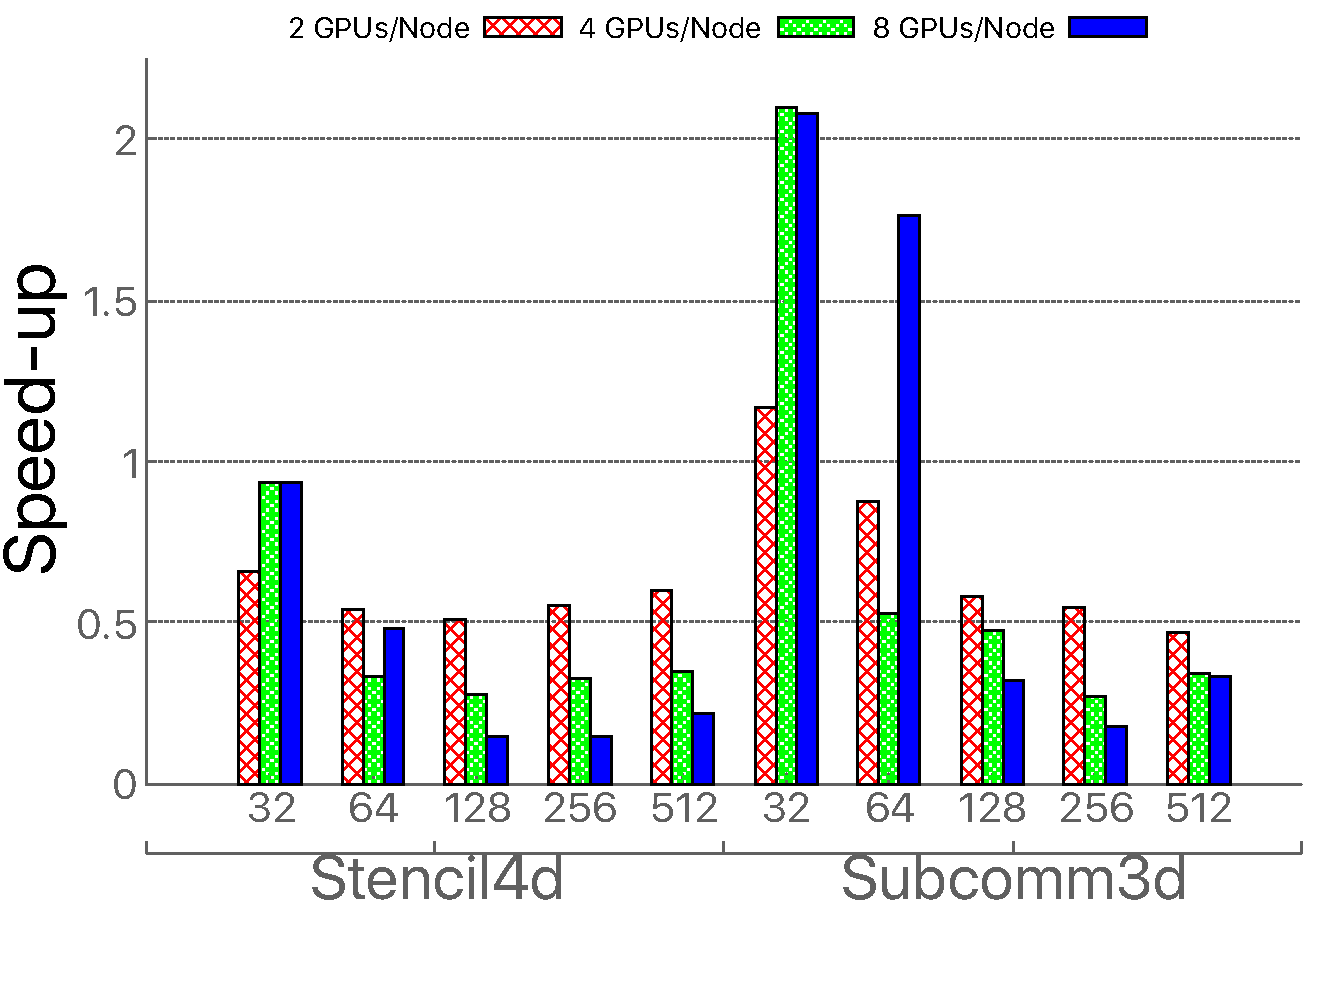
\includegraphics[width=0.3\linewidth]{plots/dfly/map/dfly-x-mapping-comm.pdf}
%  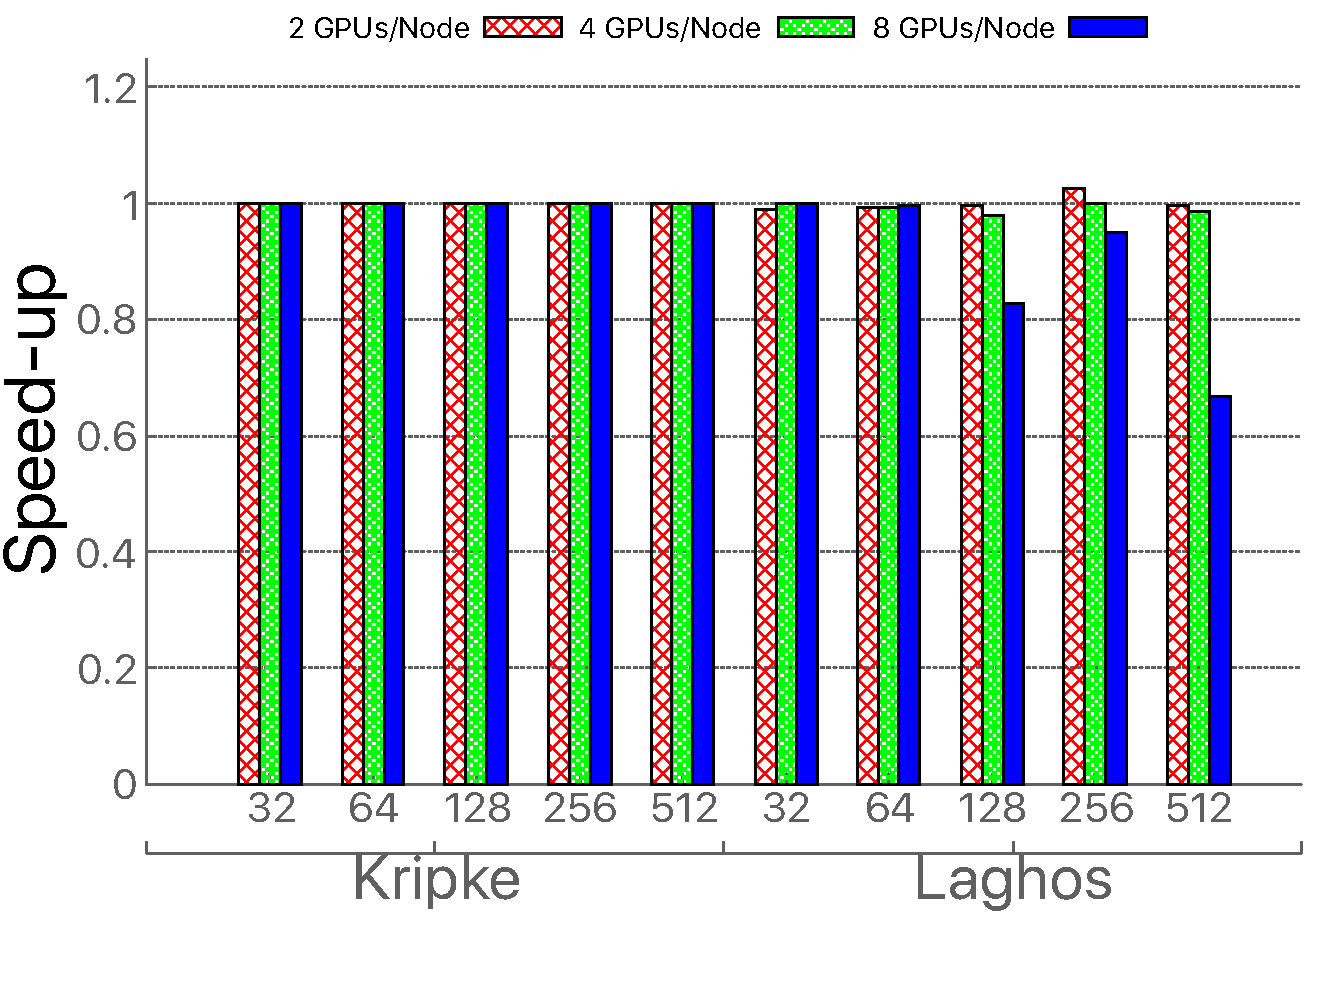
\includegraphics[width=0.3\linewidth]{plots/dfly/map/dfly-x-mapping-comp.pdf}
%  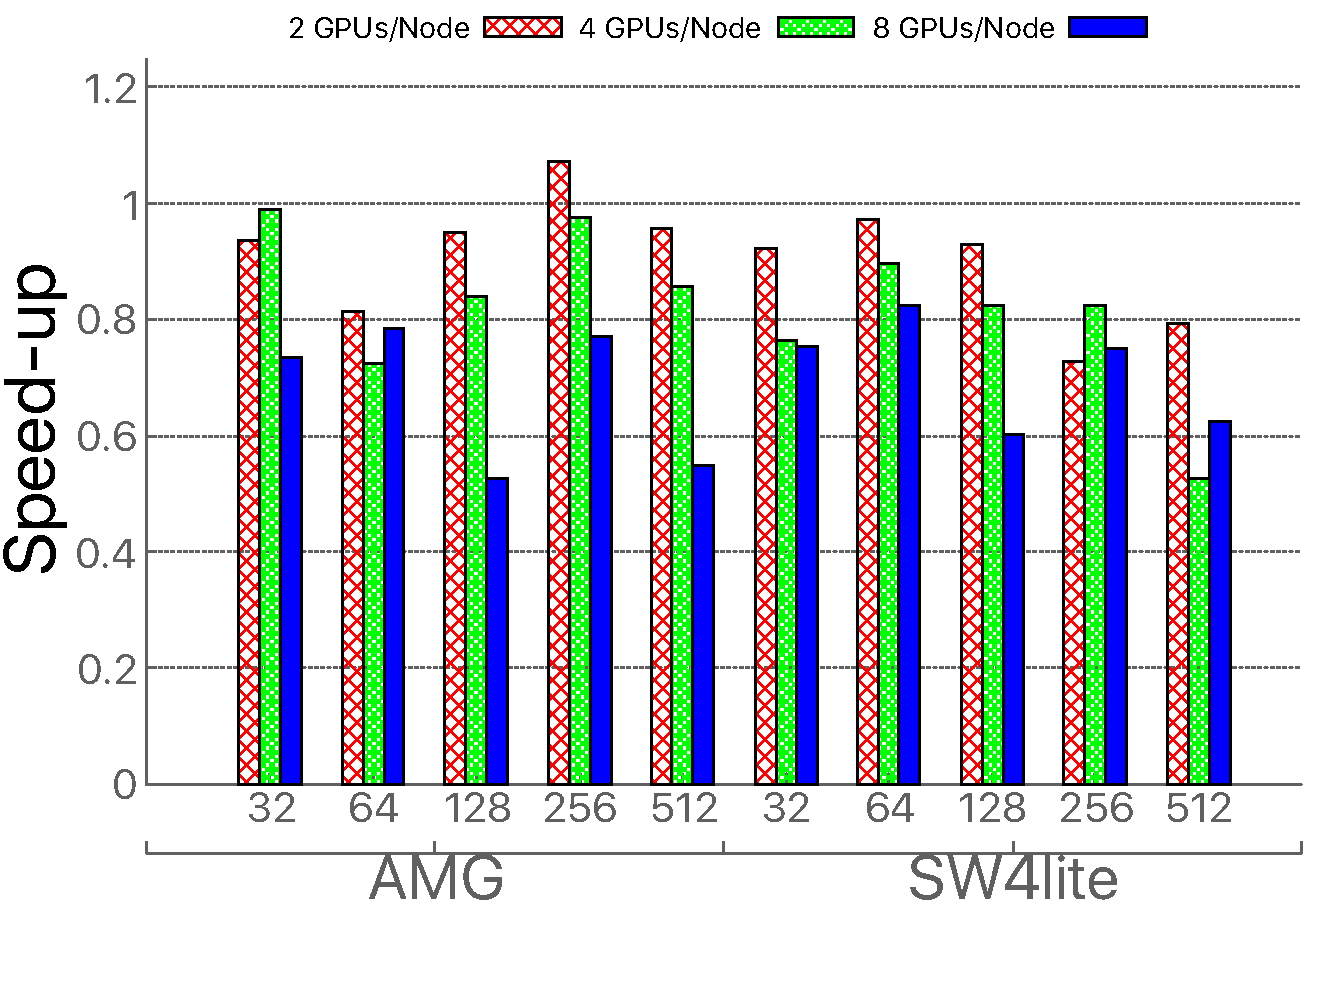
\includegraphics[width=0.3\linewidth]{plots/dfly/map/dfly-x-mapping-comp-new.pdf}
%%\end{multicols}
%\caption{Application Performance on Dragonfly with default setting and different GPU's per node}
%\end{figure}

\subsection{Impact of network bandwidth}

In the previous section, I saw that as the number of GPUs per node increases, 
the default 1x network bandwidth becomes a performance bottleneck for many
cases.  Thus, I next study the impact of varying network bandwidth along with number of
GPUs/nodes on application performance. 

\begin{figure*}[t]
\centering
    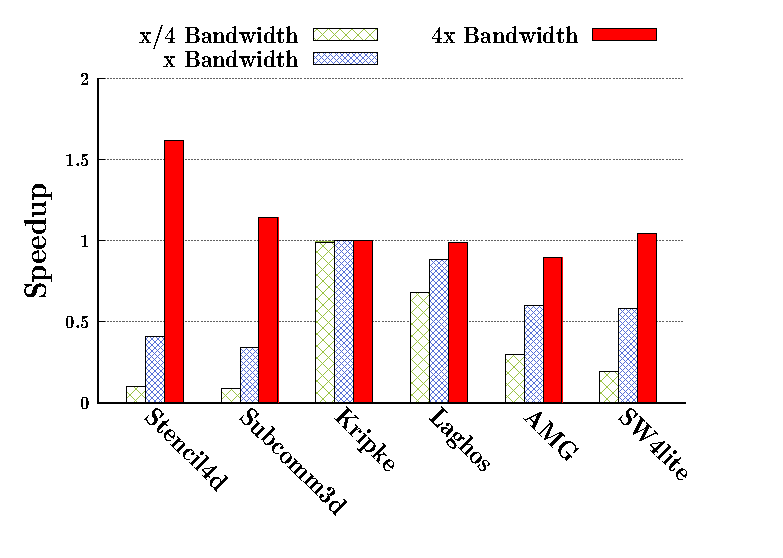
\includegraphics[width=0.8\columnwidth]{figure/plots/bw/ftree-bw-mapping-all.eps}
  \caption{Speedup for the 4 GPUs/node configuration over 1 GPU/node in fat-tree, 1x network
  bandwidth configuration. Data is shown only for job sizes of 128 GPUs.}
  \label{fig:bw_ftree}
\end{figure*}

\begin{figure*}[t]
\centering
    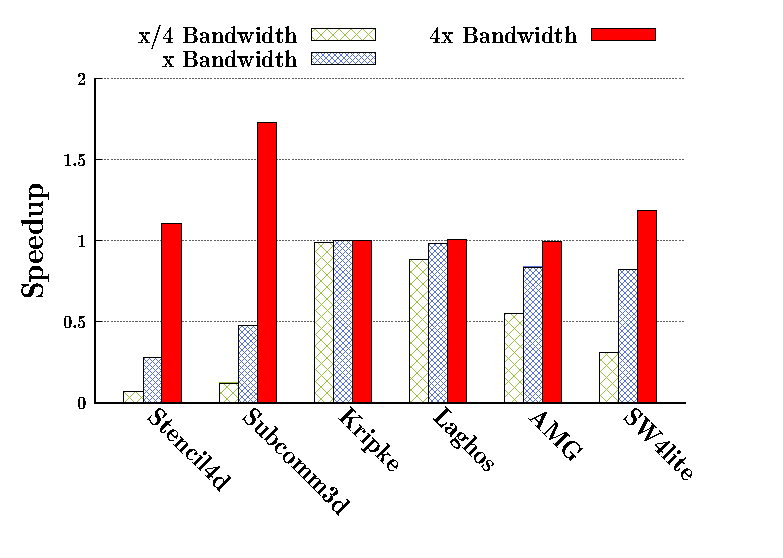
\includegraphics[width=0.8\columnwidth]{figure/plots/bw/dfly-bw-mapping-all.eps}
  \caption{Speedup for the 4 GPUs/node configuration over 1 GPU/node in 1D dragonfly, 1x network
  bandwidth configuration. Data is shown only for job sizes of 128 GPUs.}
  \label{fig:bw_dfly}
\end{figure*}

In our simulation experiments, I observed that the impact of network bandwidth on jobs of different sizes
shares similar trends. Hence, I present data only for a job size of 128 processes.
Figure~\ref{fig:bw_ftree} shows the performance for the 4 GPUs per node
configuration with varying network bandwidth relative to 1 GPU per node, 1x
network bandwidth configuration on fat-tree network. We find that the network
bandwidth has a significant impact on most applications.  The gains are  highest
for communication-heavy applications such as Stencil4d and Subcomm3d.
Conversely, the impact of reducing the network bandwidth is also highest for
those.  A similar trend is observed for the 1D dragonfly topology as
shown in Figure~\ref{fig:bw_dfly}.

Table~\ref{tab:bw_ftree} presents the minimum bandwidth required for each
application and a given job size to achieve 90\% of the performance of the
default setting for the fat-tree topology.  As expected, different types of
applications have different bandwidth requirements. In general,
communication-intensive applications require larger bandwidth to sustain the
increased number of GPUs per node while computation-intensive applications have
less bandwidth requirement. For example, for the 8 GPUs per node case with 512 processes
job size, Stencil4d needs 8x network bandwidth
to achieve 90\% of the performance from the default setting; AMG and SW4lite need more than 
4x bandwidth while
Kripke only needs x/8 bandwidth. 

\begin{table}[t]
  \centering
  \caption{Minimum bandwidth required to achieve 90\% of the performance of the
  default 1 GPU/node configuration for fat-tree}
    \label{tab:bw_ftree}
    \vspace{-1em}
    \resizebox{\columnwidth}{!}{%
    \begin{tabular}{lcccc} \toprule
\multirow{2}{*}{Applications}
 & \multicolumn{2}{c}{32 processes}  & \multicolumn{2}{c}{512 processes} \\
\cline{2-5}
& 4 GPUs/node & 8 GPUs/node & 4 GPUs/node & 8 GPUs/node  \\ \midrule
Stencil4d & 1x & 1x & 4x & 8x\\
Subcomm3d & x/2 & x/2 & 4x & 4x\\
Kripke & x/16 & x/16 & x/8 & x/8\\
Laghos & x/2 & 2x & x & 2x\\
AMG & 4x & 8x & 4x & 8x\\
SW4lite & 2x & 2x & 2x & 4x\\ \bottomrule
\end{tabular}
}
\end{table}

Further, application requirement is also affected by the job size and the
placement with other jobs.  For example, 32-process Laghos ran slower in some
workloads when mapped in the 8 GPUs per node configuration, which is why here I
need double bandwidth to get more than 90\% speedup. We also see that sometimes
communication-intensive applications such as Stencil4d and Subcomm3d require
less bandwidth in 8 GPUs per node configuration than 4 GPUs per node
configuration to reach 90\% of the performance for 32 processes and 64 processes.  This
is mainly due to the fact that, with a larger number GPUs per node, a significant
fraction of the communication happens within the same node.  This indicates that
future GPU-based platforms must consider its workloads to decide important
networking hardware parameters.  The results for 1D
dragonfly, which has a similar trend as that in fat-tree. 


\vspace{1em}
\noindent
{\it \textbf{Overall Observation}:
Bandwidth requirement to sustain high performance depends on GPU density
and job sizes.}

\noindent
Our results show that
  each type of application has a sweet-spot for them to perform effectively. 
  Hence, the design of a future GPU cluster should take its applications into
  consideration in order to achieve the maximum performance-cost ratio. 
  %Larger bandwidth allocation compensates slowdown when application is run with more GPUs per node.




\subsection{Impact of message scheduling in the NIC}

The impact of message scheduling on system performance has not received
sufficient attention in the community. To our knowledge, this is the first time
that the impact of message scheduling on system and application performance
is being studied systematically.
%The results for application with different numbers of processes have a
%similar trend.
Similar to the impact of the number of GPUs per node and network link bandwidth, the impact
of message scheduling is similar for both fat-tree and 1D dragonfly. Thus, I only discuss
results for the 1D dragonfly in detail. 

%{\bf Sap: check all numbers in this section}
\begin{figure}[t]
  \centering
  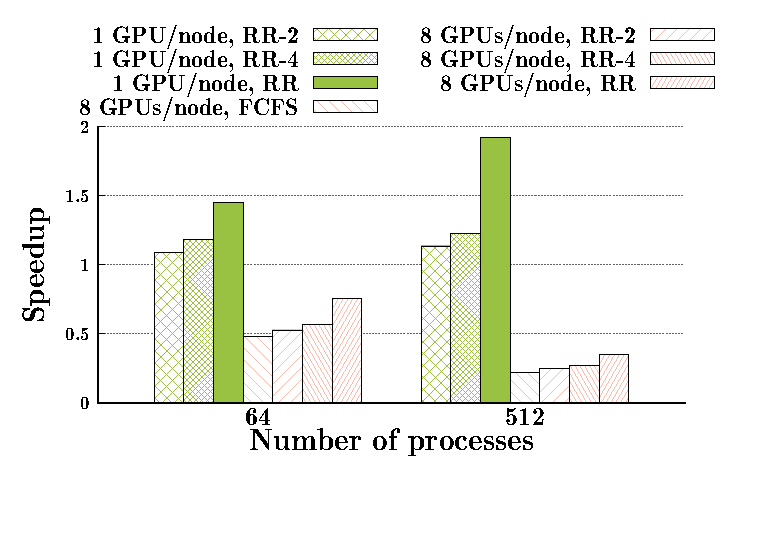
\includegraphics[width=0.8\columnwidth]{figure/plots/sched/dfly-sched-mapping-stencil.eps}
  \vspace{-0.5in}
  \caption{Results for Stencil4d (64 processes and 512 processes on 1D dragonfly)}
  \label{fig:stencil_scheduling_dfly}
\end{figure}


Figure ~\ref{fig:stencil_scheduling_dfly} shows the speedup for 64 and 512
processes (GPUs) of Stencil4d relative to the default case with 1 GPU per node and
FCFS scheduling (network bandwidth is fixed at 1x for all configurations).  For
the 1 GPU per node cases, the scheduling significantly affects the performance:
the larger the number of messages the scheduler considers for packetization
concurrently, the higher the performance. The RR scheduler reaches a speed-up of
1.45 for the 64-process job and 1.93 for the 512-process job in comparison to
the default FCFS scheduler. A similar trend is observed for the 8 GPUs per node
cases: the RR scheduler improves the speed up from 0.48 with the FCFS scheduler to 0.76
for the 64-process job, and from 0.22 to 0.35 for the 512-process job. 

\begin{figure}[t]
\centering
  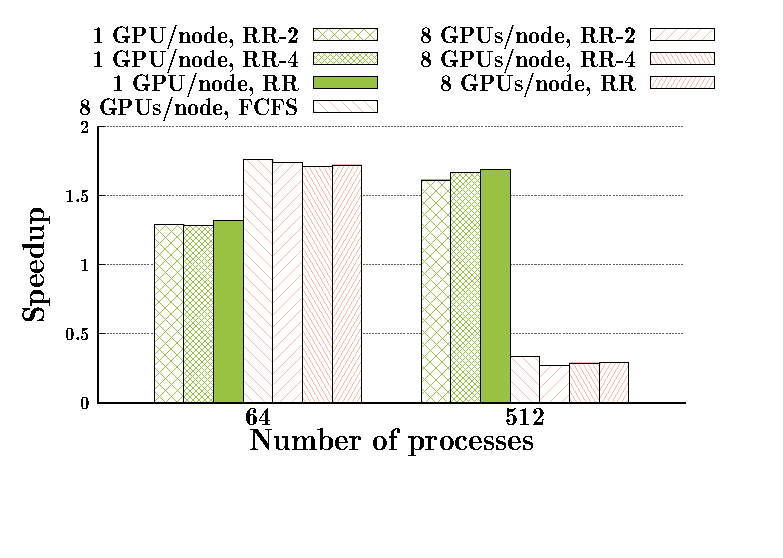
\includegraphics[width=0.8\columnwidth]{figure/plots/sched/dfly-sched-mapping-subcom.eps}
  \vspace{-0.5in}
  \caption{Results for Subcomm3d (64 processes and 512 processes on 1D dragonfly)}
  \label{fig:subcomm3d_scheduling_dfly}
\end{figure}


Figure ~\ref{fig:subcomm3d_scheduling_dfly} shows the speedup for 64 and 512
processes of Subcomm3d.  For 1 GPU per node, RR scheduler performs better
than FCFS. However, RR is only slightly better than RR-2 and RR-4 and achieves a
1.3 speed-up for the 64-process job and 1.7 speed-up for the 512-process job
over FCFS.  For 8 GPUs per node cases, all schedulers have similar performance
with FCFS being slightly better than other scheduling schemes. Although both
Stencil4d and Subcomm3d are communication-intensive, the impact of message
scheduling is different. This is because the communication characteristics in
these two applications are different. 

\begin{figure}[t]
  \centering
  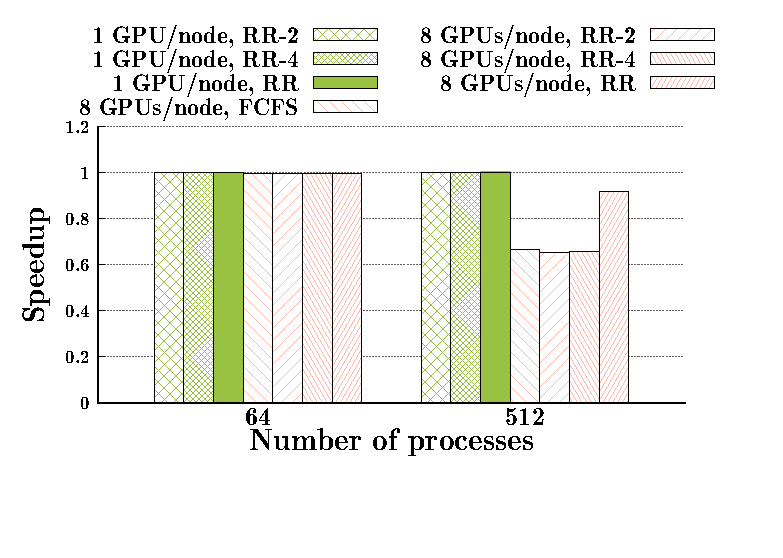
\includegraphics[width=0.8\columnwidth]{figure/plots/sched/dfly-sched-mapping-laghos.eps}
  \vspace{-0.5in}
    \caption{Results for Laghos (64 processes and 512 processes on 1D dragonfly)}
  \label{fig:laghos_scheduling_dfly}
\end{figure}


Message scheduling has no impact on Kripke as Kripke is not sensitive to
communication as seen earlier. Figure~\ref{fig:laghos_scheduling_dfly} shows
the speedup for 64-process and 512-process simulations of Laghos. For 1 GPU per node cases, all
schedulers have the same performance. For 8 GPUs per node cases, all schedulers
have the same performance for the 64-process job, but RR has a significantly
better performance than others for the 512-process job. As shown in
Figure~\ref{fig:dfly_gpu}, for 512 processes (and 256 processes and 128
processes), Laghos is affected by communication only in the 8 GPUs per node
setting.

%\begin{figure}[h]
%  \centering
%  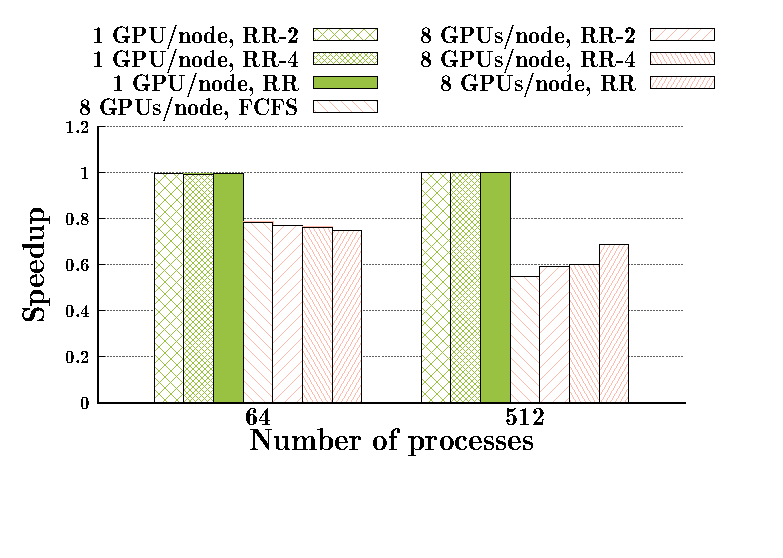
\includegraphics[width=\columnwidth]{figure/plots/sched/dfly-sched-mapping-amg.eps}
%  \vspace{-0.5in}
%    \caption{Results for AMG (64 processes and 512 processes on 1D dragonfly)}
%  \label{fig:amg_scheduling_dfly}
%\end{figure}

\begin{figure}[t]
  \centering
  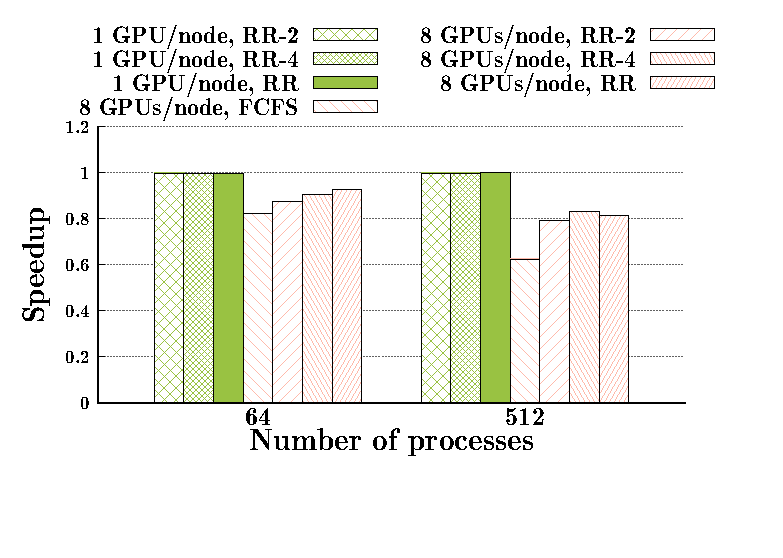
\includegraphics[width=0.8\columnwidth]{figure/plots/sched/dfly-sched-mapping-sw4lite.eps}
  \vspace{-0.5in}
  \caption{Results for SW4lite (64 processes and 512 processes on 1D dragonfly)}
  \label{fig:sw4lite_scheduling_dfly}
\end{figure}


Figures~\ref{fig:sw4lite_scheduling_dfly} show the
results for SW4lite. Message scheduling has no impact on the 1 GPU per node cases, but
affects the performance significantly for 8 GPUs per node cases for both applications and the two
job sizes. The impact, however, depends on both the application and job sizes.
Simillar results are seen for AMG application.
%This is due
%to the changing of the inter-node communication characteristics. Simillar results are seen for AMG.

\vspace{1em}
\noindent
{\it \textbf{Overall Observation}:
For most applications, some degree of round robin in NIC scheduling is effective. However
    the exact degree is application dependent -- no single scheduling scheme can achieve the best
  performance across applications.}

Message scheduling can impact performance only when there are many concurrent
communicating pairs. For the 1 GPU per node cases, it thus only affects the
communication heavy applications such as Stencil4d, and has virtually no impact
on the other applications in our study. As the number of GPUs per node
increases, so does the  number of communication sources and the number of
concurrent communications. Thus, with 8 GPUs per node, message scheduling makes
a difference in all applications, except Kripke.  The magnitude of the impact,
however, depends on the application as well as the job size: Round-robin (RR) is
the most effective scheduling in many cases.  However, each of the scheduling
schemes that I use in our study achieves the best performance in some cases.
For example, FCFS is the best for AMG with 64 processes and 8 GPUs per node;
RR-4 is slightly better than other scheduling policies for SW4lite with 512
processes and 8 GPUs per node.  We conclude that the effectiveness of message
scheduling depends on both application and the network parameters, and needs to
be further studied by examining more applications as well as system
configurations. 





\section{Summary}
This chapter explored the intricate dynamics of optimizing hardware parameters for future GPU-based High Performance Computing (HPC) platforms. The study identified that the integration of multiple GPUs per compute node, a trend driven by the need for increased computational capacity, necessitates a reevaluation of traditional hardware configurations. The core of this investigation is the development of a comprehensive simulation study using the TraceR-CODES tool, focusing on three pivotal hardware parameters: the number of GPUs per node, network link bandwidth, and network interface controller (NIC) scheduling policies. This study is contextualized within the frameworks of two prevalent network topologies: fat-tree and dragonfly.
The findings from this research challenge the conventional wisdom on HPC platform optimization. It is revealed that the interplay between hardware parameters and application performance is nuanced, requiring a tailored approach to system design. Particularly, the study unveils that the optimal configuration of GPUs per node significantly hinges on the specific demands of the applications running on the platform. For communication-intensive applications, enhancing network bandwidth is critical for sustaining performance as the number of GPUs per node increases. Conversely, computation-heavy applications exhibit a different sensitivity pattern to network bandwidth variations but are influenced by the strategies employed for NIC scheduling.
Moreover, the work introduces a novel perspective on the role of hardware parameters in shaping HPC system performance. The simulation results indicate that a holistic approach, which meticulously balances computational capacity with communication efficiency through strategic hardware parameter configuration, is imperative for the design of future GPU-based HPC platforms.
By dissecting the complex relationship between hardware parameters and system performance, it lays the groundwork for designing more powerful, efficient, and capable HPC platforms, thereby addressing the evolving demands of high-performance computing applications.
In the following chapter, I apply this groundwork and select specific hardware parameters which can optimally run HPC applications in a state-of-the-art HPC environment for evaluating SDN-enhanced routings.
